\section{Law amendments and the KBP}
\label{law}

%As suggested by \cite{Bench-Capon1992} we started the formalization of the domain with the creation of an intermediate representation of the domain.
As the former version of the legislation concerning registration duties  was unstructured and difficult to read, the model was built on more accessible information from the Federal Public Service Finance \cite{FODFinancien}. 
We analyzed and formalized the domain using the Decision Model and Notation (DMN) methodology.\footnote{The reasons and way of working with DMN are discussed in our earlier work, see \cite{ruleml/DeryckHVV18}.}
This resulted in a model consisting of a glossary and multiple connected decision tables. 
This was then translated into the IDP-language.
The result is an initial prototype that formalizes 11 articles of law, resulting in a knowledge base of 53 concepts, 6 constraints and 14 rules \cite{ruleml/DeryckHVV18}. Building this knowledge base required an effort of approximately 10 person-days.
A significant part of this time was attributed to the creation of the set of symbols representing concepts in the domain (i.e. the \emph{vocabulary}. %In this phase some design choices need to be made, e.g., use of \emph{reification} for auxiliary concepts, or the choice between the use of a function or a relation.  
To this end some analysis beyond the level of the DMN model was needed.

To evaluate the maintainability of the knowledge base, we examined the effort necessary to update it to the changes in legislation enacted in 2018. 
These changes consisted of 5 new articles, making it the most significant change to real estate sales law since the transfer of jurisdiction from the national to the Flemish regional government in 2013. %\footnote{The decree of July 17 2015 made small amendments to a larger number of articles, but only introduced 3 new articles.} 
At the time of constructing the original knowledge base, the content of these changes was not yet known.
Therefore, this provides a realistic test case to judge the maintainability of the knowledge base.

Updating the knowledge base required only $0.5$ person-days, a fraction of the time required for the initial version. 
16 of the original 53 concepts were removed and 18 new ones added; 11 existing constraints and rules needed to be updated or deleted, while 4 new constraints were added. 
Crucially, 9 of the 20 existing constraints/rules did not need to be touched at all. 
This demonstrates that the inherent modularity of the KBP indeed leads to significant advantages in practice.

\begin{comment}


To give an idea of the required changes, we briefly discuss an example.

%that were required to the knowledge base, we briefly provide some examples.
%The dependency between the \textit{kadastral income} and the number of children as demonstrated in figure \ref{fig:old} is formalized in the definition below.
%As the concept of \textit{kadastal income }is eliminated in the new law, this piece of code is deleted in the new program.
%\begin{align*}
%\{ & MaxKi = 745 \leftarrow 0 \leq NmbChildren \leq 2. \\
%& MaxKi = 845 \leftarrow 3 \leq NmbChildren \leq 4.\\
%& MaxKi = 945 \leftarrow 5 \leq NmbChildren \leq 6.\\
%& MaxKi = 1045 \leftarrow 7 \leq NmbChildren. \}
%\end{align*}
In the original prototype, the $RegistrationType$ is defined by a number of rules such as:
%Determination of the registration type is modelled as a definition with multiple rules in which the defining rules from the different types are described. 
%For the legislation prior to June 2018, the structure of the definition was the following (the formulas representing the effective conditions are abstracted and represented by \textit{conditionsOld} resp. \textit{conditionsNew}):
\[\left\{\begin{aligned}
 RegistrationType = Social &\leftarrow \varphi_1.\\
 RegistrationType = Modest &\leftarrow \varphi_2.\\
& \cdots
\end{aligned}\right\}\]
%& HasRegistrationType = commercialPurchase \leftarrow conditionsOld.\\
%& HasRegistrationType = other \leftarrow HasRegistrationType \neq socialDwelling \\
%& \indent \wedge HasRegistrationType \neq modestDwelling\\
%& \indent \wedge HasRegistrationType \neq commercialPurchase. \}
%\end{align*}
After the amendments, new registration types needed to be added (e.g., $Monument$), while some disappeared (e.g., $Modest$) and others remained unchanged (e.g., $Social$).
Thanks to the modular nature of rule-based definitions, these correspond to local changes that preserve the global structure of the definition:
\[\left\{\begin{aligned}
 RegistrationType = Social &\leftarrow \varphi_1.\\
 RegistrationType = Monument &\leftarrow \varphi'.\\
& \cdots
\end{aligned}\right\}\]
%\begin{align*}
%\{ & RegistrationType = socialDwelling \leftarrow conditionsOld.\\
%& HasRegistrationType = familyDwelling \leftarrow conditionsNew.\\
%& HasRegistrationType = withEnergyRenovation \leftarrow %conditionsNew.\\
%& HasRegistrationType = monument \leftarrow conditionsNew.\\
%& HasRegistrationType = commercialPurchase \leftarrow conditionsOld.\\
%& HasRegistrationType = other \leftarrow HasRegistrationType \neq socialDwelling \\
%& \indent \wedge HasRegistrationType \neq familyDwelling\\
%& \indent \wedge HasRegistrationType \neq withEnergyRenovation\\
%& \indent \wedge HasRegistrationType \neq monument\\
%& \indent \wedge HasRegistrationType \neq commercialPurchase. \}
%\end{align*}
%\jo{Hebben we effectief de accolades rond de rules nodig?}
%\Marjolein{naar analogie met de voorbeelden in sectie 3 zou ik dit wel doen}
%The initial analysis of the domain took a considerable amount of time, as the modeller did not have any prior domain knowledge.
%Note that, especially with the approach used, the prior analysis of the domain and its formalization with the use of DMN could be done by a domain expert \cite{iets over DMN en gebruik door business users}.
%However, some additional analysis and understanding of the domain by the \idp-modeller is needed, as certain formulation choices impact the way variables are presented by the interface \cite{Marjolein}.

%Typical for the former regulation was the use of multiple versions of the same concept at different law articles.
%E.g., the definition of 'first property' and the establishment obligation were interpreted differently in the context of the type of real estate (TRE) and the context of abattement.
%\begin{sidewaysfigure}
%\begin{figure}[h]
%    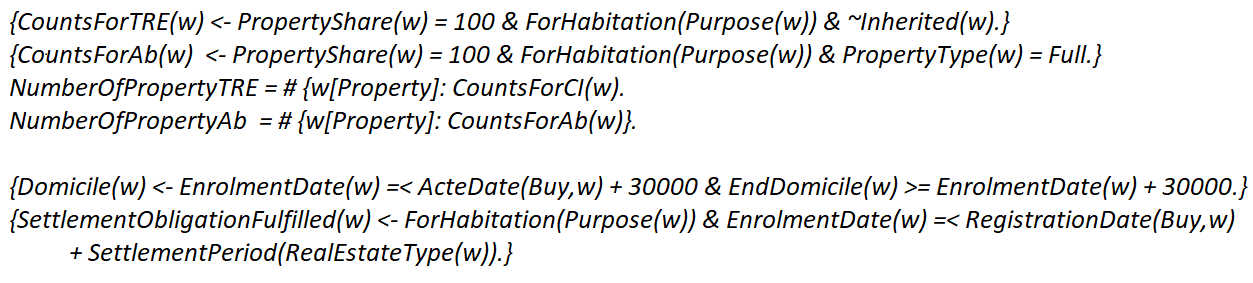
\includegraphics[angle=0,width = 1\linewidth]{img/codeOld.png}
  	%\caption{geen captation:voorbeeldcode.}
%	\label{fig:code}
%\end{figure}
%\end{sidewaysfigure}
%\jo{What is the purpose of this code?}

%\subsubsection{Regulation as from June 1st 2018}
%As discussed above, the regulation changed considerably as from June 1st 2018.
%In our application we modelled the new regulation (without transitional measures for transactions concluded prior to June 1st but registered after this date).
%One of the claims of KBP is that it allows agile adaptations, as all and only conditions are centralized in the concise knowledge base.
%It took a half day of work to implement the profound changes that were described in \ref{sec:background}: two hours were needed to search, analyze and model the new legislation using DMN; and an additional hour and a half were needed to amend the IDP-code. %exacte timings opzoeken%

\end{comment}